\documentclass[laboratorio]{guia}

\def \practnum {6} 
\def \practica {Circuito RLC: resonancia en serie y en paralelo}

\def \materia {Laboratorio de F\'\i sica II para Qu\'\i micos}
\def \periodo {2\sptext{o} cuatrimestre de 2016}
\def \profesor {Diana Skigin}
\def \website {http://materias.df.uba.ar/f2qa2016c2}
 
\usepackage{graphics}
\usepackage{amsmath}
\usepackage{amsfonts}
\usepackage{graphicx}
\usepackage{float}
\usepackage{wrapfig}
\usepackage{subfigure}
\usepackage{bm}
\usepackage{grffile}
\usepackage{color}
\usepackage{framed}
\usepackage[utf8]{inputenc}
\usepackage[T1]{fontenc}
\usepackage{lmodern} 
% definicion del entorno 'sabermas'
\makeatletter
\definecolor{shadecolor}{rgb}{0.89,0.91,0.94}
\newenvironment{sabermas}[1]{%
\vfill
\begin{shaded}
  \begin{center}
  {\textsection{Para saber m\'as}}
  \end{center}
  #1
\sf } 
{%
\end{shaded}%
}
\makeatother

\renewcommand{\vec}[1]{\ensuremath{\mathbf{#1}}}




\hyphenation{ coe-fi-cien-tes coe-fi-cien-te au-to-va-lor
              au-to-va-lo-res co-rres-pon-der pro-ble-ma 
              cual-quie-ra po-la-ri-za-cio-nes }

\graphicspath{{./Guia_06_Circuito_RLC/}}

\begin{document} 
\objetivo{Determinar experimentalmente la frecuencia de resonancia en un circuito
RLC serie y paralelo. Estudiar adem\'as el desfasaje entre la tensi\'on y la 
corriente en funci\'on de la frecuencia de operaci\'on del circuito.   
\tematicas{Circuitos de corrientes variables en el tiempo, RLC, resonancia.}} 
\maketitle

\section{Circuito RLC serie}

\subsection{Introducci\'on}

Considere el circuito RLC mostrado en la Figura \ref{fig:circuitoRLCserie}, en el
cual un capacitor $C$, una inductancia $L$ y una resistencia
$R$, se encuentran conectados en serie a un generador
de funciones $G$.

Aplicando las leyes de Kirchoff al circuito de la figura, 
tenemos:
\begin{equation}
    V_G = V_L + V_R + V_C = L \frac{dI}{dt} + RI + \frac{q}{C},
\end{equation}
ecuaci\'on que podemos derivar nuevamente para obtener
\begin{equation}
    \frac{dV}{dt} = L \frac{d^2I}{dt^2} + R \frac{dI}{dt} + \frac{I}{C}.
\end{equation}

Si el voltaje suministrado por el generador $G$ es sinusoidal, entonces el 
t\'ermino a la izquierda de la \'ultima ecuaci\'on es
\begin{equation}
    V(t) = V_m \sin \left( \omega t \right),
\end{equation}
y la corriente circulante por el circuito estar\'a dada por
\begin{equation}
    I(t) = I_m \sin \left( \omega t + \phi \right),
\end{equation}
siendo $\omega = 2\pi f$ la frecuencia angular, y $f$ la frecuencia 
(medida en Hz) suministrada por el generador de funciones. 

La impedancia $Z$ del circuito es 
\begin{equation}
    Z = Z_R + Z_L + Z_C = R + j \left( \omega L - \frac{1}{\omega C} \right),
\end{equation}
siendo $j$ la unidad imaginaria, por lo que
\begin{equation}
    V = IZ = I \left[ R + j \left( \omega L - \frac{1}{\omega C} \right) \right].
\end{equation}

Ahora bien, la tangente del \'angulo de desfasaje entre tensi\'on y corriente
ser\'a igual al cociente entre las partes imaginaria y real de la impedancia
$Z$, es decir:
\begin{equation}
    \tan \left( \phi \right) = \frac{\text{Im} Z}{\text{Re} Z} = 
    \frac{1}{R} \left(\omega L - \frac{1}{\omega C} \right),
\end{equation}
y el m\'odulo de la impedancia, resultar\'a
\begin{equation}
    |Z|^2 = R^2 + \left( \omega L - \frac{1}{\omega C} \right)^2.
\end{equation}

El \'angulo de desfasaje $\phi$ entre $I$ y $V$ puede ser positivo, en cuyo
caso el circuito es capacitivo. Si, por el contrario, $\phi < 0$, se dice que
el circuito es inductivo. Finalmente, si no hay desfasaje entre corriente y 
tensi\'on, el circuito se denomina resistivo. En este \'ultimo caso, tensi\'on
y corriente est\'an en fase y la parte imaginaria de la impedancia es nula.
Esta condici\'on implica
\begin{equation}
    \omega L - \frac{1}{\omega C} = 0,
\end{equation}
condici\'on que se cumple para la denominada {\it frecuencia de resonancia} 
$\omega_0$:
\begin{equation}
    \omega_0 = \frac{1}{\sqrt{LC}}.
\end{equation}
Resulta f\'acil observar que, para este caso, la corriente circulante por 
el circuito alcanza su amplitud m\'axima. En este marco, definimos el 
{\it ancho de banda} $\Delta \omega$ como el intervalo de frecuencias para
el que la potencia disipada disminuye exactamente a la mitad de la m\'axima
potencia disipada. De acuerdo a nuestros resultados anteriores, el 
ancho de banda para el circuito RLC serie viene dado por
\begin{equation}
    \Delta \omega = \frac{R}{L}.
\end{equation}
Definiendo ahora el {\it factor de calidad} o {\it m\'erito} $Q$ mediante
\begin{equation}
    Q = \frac{\omega_0}{\Delta \omega},
\end{equation}
obtenemos, para el caso del circuito que nos ocupa:
\begin{equation}
    Q = \frac{\omega_0 L}{R}.
\end{equation}

\subsection{Desarrollo de la experiencia}

En esta parte de la pr\'actica, se propone montar un circuito como el de la
Figura~\ref{fig:circuitoRLCserie}. A continuaci\'on:
\begin{enumerate}
    \item Estudie la variaci\'on de la tensi\'on sobre la resistencia en 
        funci\'on de la frecuencia de operaci\'on. 
    \item A partir de las mediciones realizadas en el inciso anterior,
        encuentre la frecuencia de resonancia y el valor del factor de
        calidad. Recuerde que la inductancia tiene una resistencia propia 
        (tal y como se muestra
        en la Figura~\ref{fig:circuitoRLCserie}) y, seg\'un corresponda,
        deber\'a ser considerada en la resistencia total del circuito.
    \item Determine experimentalmente el desfasaje $\phi(\omega)$ en funci\'on 
        de la frecuencia; para lo cual puede resultarle \'util el {\it modo XY}
        del osciloscopio. Para m\'as informaci\'on, consulte el apunte acerca
        de {\it C\'omo determinar el desfasaje entre dos se\~nales}.
\end{enumerate}

\begin{figure}[t!]
    \centering
    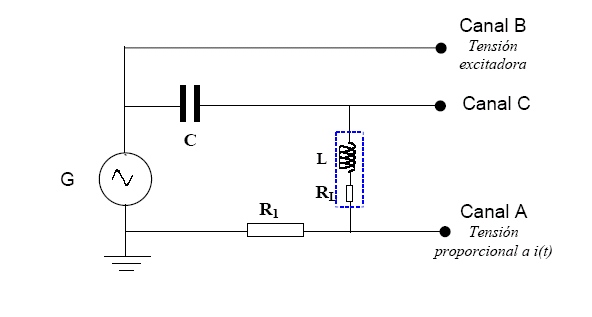
\includegraphics[width=9cm]{LG06--000.png}
    \caption{Esquema del circuito RLC serie.}
    \label{fig:circuitoRLCserie}
\end{figure}

\section{Circuito RLC paralelo}

\subsection{Introducci\'on}

Considere ahora el circuito RLC paralelo cuyo esquema se ilustra en la 
Figura~\ref{fig:circuitoRLCparalelo}. Comience por analizar te\'oricamente
esta nueva configuraci\'on con las herramientas matem\'aticas empleadas
en la primera parte de la pr\'actica. 

En este circuito, la impedancia viene dada por la impedancia del paralelo
$(L,C)$, que llamaremos $Z_{LC}$, en serie con la impedancia de la resistencia,
$R$. Dado que la inductancia tiene una resistencia interna $R_L$, tenemos 
\begin{equation}
    \frac{1}{Z_LC} = \frac{1}{Z_C} + \frac{1}{R_L+Z_L},
\end{equation}
es decir,
\begin{equation}
    Z_{LC} = \frac{ \left( R_L + j \omega L \right) \left( -\frac{j}{\omega C}  \right)   }{R_L + j \left( \omega L - \frac{1}{\omega C}\right)}.
\end{equation}
Para desfasaje nulo ($\phi = 0$), habr\'a un m\'\i nimo en la potencia
transferida cuando la frecuencia angular sea igual a
\begin{equation}
    \omega_0' = \frac{1}{\sqrt{LC}} \sqrt{1 - R_L^2 \frac{C}{L}}.
\end{equation}
Observe que si la resistencia interna de la inductancia resulta nula, entonces
\begin{equation}
    \omega_0' = \frac{1}{\sqrt{LC}}.
\end{equation}

\subsection{Desarrollo de la experiencia}

Para esta segunda parte de la pr\'actica, comience por montar el 
circuito de la
Figura~\ref{fig:circuitoRLCserie}. A continuaci\'on:
\begin{enumerate}
    \item Estudie la variaci\'on de la tensi\'on sobre la resistencia en 
        funci\'on de la frecuencia de operaci\'on. 
    \item A partir de las mediciones realizadas en el inciso anterior,
        encuentre la frecuencia de antiresonancia y el valor del factor de
        calidad.     
    \item Determine experimentalmente el desfasaje $\phi(\omega)$ en funci\'on 
        de la frecuencia; para lo cual puede resultarle \'util el {\it modo XY}
        del osciloscopio. Para m\'as informaci\'on, consulte el apunte acerca
        de {\it C\'omo determinar el desfasaje entre dos se\~nales}.
    \item Compare los resultados de esta parte con aquellos obtenidos en el
        estudio del circuito RLC serie.
\end{enumerate}

\begin{figure}[t!]
    \centering
    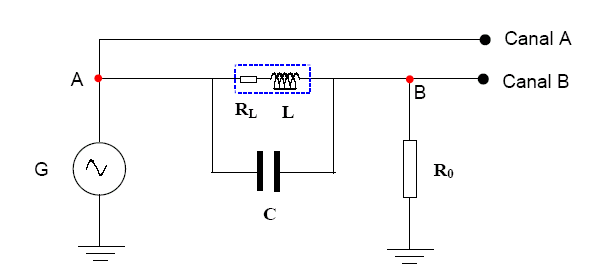
\includegraphics[width=9cm]{LG06--001.png}
    \caption{Esquema del circuito RLC paralelo.}
    \label{fig:circuitoRLCparalelo}
\end{figure}

\nocite{Alonso1998,Crawford1994,Purcell1988,Reitz1996,Trelles1984,Reitz1996}
\bibliographystyle{unsrt} 
\bibliography{Bibliografia}


\end{document}
